\documentclass [a4j,11pt] {jsarticle}

\title  {大規模社会ネットワークからのクラスタ構造の抽出\thanks {
  この論文は鶴見敏行さんが東京工業大学理学部情報科学科の学士論文研究を国際学会で
  発表した論文 \protect\cite {wakita-2007-finding-community-structure-in-mega-scale-social}を
  もとに情報リテラシの実習教材に作り直したものです。}}
\author {鶴見 敏行\thanks {東京工業大学大学院数理・計算科学専攻} \and 脇田 建{$^\dagger$}}
\date {2008年6月10日}

\usepackage {amsmath} % さまざまな数式を用いるための設定
\usepackage [dvipdfmx]{graphicx,color} % 図を取り込んだり、色を利用するための設定

\usepackage [dvipdfmx, % 自動的にハイパーリンクを作成するための設定
             bookmarks=true,
             bookmarksnumbered=true,
             bookmarkstype=toc] {hyperref}
\usepackage {pxjahyper} % pLaTeXでhyperrefにおけるPDFの目次の文字化け問題を調整

\usepackage {literacy} % この実習用のためだけの特殊な設定

\begin {document}

\maketitle


\begin {abstract}
Clauset,Newman,Mooreはネットワークをボトムアップかつ貪欲に解析する手
法(CNM法)を提案し、50万ノード程度までの社会ネットワーク解析を
可能としたが、それ以上の規模については実用的な時間内での解析は困難であっ
た。そこでCNM法の合併の過程を観察した。その結果合併するクラス
タサイズの不均衡が計算コストに大きく影響していることが明らかとなった。
この観測から、合併するクラスタサイズの均衡が法の速度向上につ
ながると考えた。本稿では、合併時のクラスタのサイズを考慮することにより
合併比率を向上させる3種類の手法を提案する。提案手法の実験データセットと
して、国内最大級のソーシャルネットワーキングサービスより2006年10月に取
得した550万ユーザーの友人関係のネットワークを使用した。提案した3つの手
法を用いたところ、CNM法に比べ劇的なスケーラビリティの向上がみ
られた。もっとも速度向上がみられた手法では、100万ノードに対し
て5分、400万ノードに対しては35分程度で解析する事に成功した。また別の手
法では、50万ノードに対して50分(CNM法より7倍早い)で解析でき、
モジュール性の向上にも成功した。
\end {abstract}

\section {はじめに}
\label {sect: はじめに}

クラスタ構造の抽出は、複雑な社会ネットワークからその固有の性質を知るう
えでの最初の重要なステップであり、今までに数々の研究がなされてい
る。
\cite{Kleinberg99,
  Page99,
  Dean99,
  Kumar99,
  Miller01,
  Toyoda01,
  Wu04,
  Cai04,
  Clauset04,
  Onsjo06}


われわれは、Clauset, Newman, Moore によって提案された手法(CMM法)
\cite{Clauset04}
を実装し、Social Networking Service(SNS)より取得したネットワークのさまざまな部分集合に対しての解析を試みた。
50万ユーザー以下での解析は可能だった。
しかし、さらに大きなネットワークでは実用的な時間での解析は不可能であった。

そこでCNM法の合併の過程を観察した。その結果合併するクラスタサ
イズの不均衡が計算コストに大きく影響していることが明らかとなった。この
観測から、合併するクラスタサイズの均衡が法の速度向上につなが
ると考えた。

本稿では合併するクラスタの大きさについての不均衡を抑えるために、クラス
タサイズの比である\emph {合併比率}を定義し、合併
するクラスタの選定の基準として従来用いられてきた{\em モジュール性}
に合併比率を加味するヒューリスティックを提案する。この提案を用いて実験を
行った結果、合併の不均衡を抑えることができ、数百万ノードのネットワーク
に対する解析も可能となった。

これ以後の本稿の構成は以下の通りである。\ref
{sect: related}節で関連研究について述べる。\ref {sect: cnm}節でCNM法
を紹介し、その問題点を明らかにする。
\ref{sect: algorithm}節ではCNM法の欠点を改善するヒューリスティクを提案し、
\ref{sect: evaluation} 節では提案方法を評価する。
最後に\ref{sect: summary}節で本稿をまとめる。

\section {関連研究}
\label {sect: related}

\emph{クラスタ}を抽出する手法は大きく分けて二つある。
一つは、グラフよりいくつかのノードを\emph{種}として選び、それを含むクラスタを返す手法
\cite{Kleinberg99,Dean99,Miller01,Toyoda01}である。
もう一つは、ネットワーク全体をクラスタに分割する手法
\cite{Page99,Kumar99,Wu04,Clauset04,Cai04,Onsjo06}である。

前者の手法は主にウェブの解析に使われている。ウェブの解析は、各ウェブペー
ジをノード、ハイパーリンクを\emph {エッジ}とした有向グラフとしてウェブ
をとらえ、解析する。Kleinbergが提案した\emph {HITS} \cite{
  Gibson98,
  Kleinberg99}
は、ウェブの適当な部
分グラフの中からハイパーリンクで密に結合された\emph {オーソリティ}およ
び\emph {ハブ}を抽出する手法である。オーソリティとは、多くのペー
ジからハイパーリンクを張られている著名なページである。ハブとは、リンク
集およびブックマークなど、多くの著名なページへハイパーリンクを張ってい
るページである。HITSは、簡単な反復計算によって各ウェブページのオーソリ
ティおよびハブのスコアを計算する。

後者の手法としてさまざまな提案がなされている。Kumarらによる\emph
{Trawling} \cite{Kumar99}
は特によく知られている。彼らは、2 億ページ以上の大規
模なウェブのアーカイブに対してこの手法を適用し、10万個を越えるクラスタ
の\emph {コア}を発見した。コアとはオーソリティとハブから成るサイズの小
さい%:\emph {完全2部グラフ}:%であり,ほとんどのクラスタがコアを含むという
仮定に基づいている。Clausetらにより提案された手法(CNMアルゴリ
ズム)
\cite{Clauset04}
は、本研究と関連が深いため、次節で説明する。


\section {CNM法}
\label {sect: cnm}

\newcommand\clustering [0] {\ensuremath {{\cal C}}}
\newcommand\DQ [3] {\ensuremath {\Delta Q^{#1}_{#2,#3}}}

NewmanとGirvanは、グラフ$G$に対するクラスタ
リング$\clustering$が与えられたときに、そのクラスタリングの優劣を評価す
るための指標として\emph {モジュール性}$Q(G,\clustering)$を定義し\cite
{Newman04}
、モジュール性を指標として貪
欲にクラスタを合併する手法を提案した。のちにClauset,Newman,Mooreらは
それにデータ構造上の改善を施した案を提案した(CNM法)
\cite{Clauset04}。

CNM法では、まずそれぞれのノードを独立したクラスタとして表す。
そして、全クラスタ対$(c_i, c_j)$について、それらを合併したときのモジュー
ル性の上昇度($\DQ \clustering {c_i} {c_j}$)を計算する。ここで$
\DQ \clustering {c_i} {c_j}$の定義は以下の通りである。
%
\[ \DQ \clustering {c_i} {c_j} =
   Q(G,\clustering \setminus \{c_i, c_j\} \cup \{c_i \cup c_j\}) -
   Q(G, \clustering). \]


CNM法は、最大値を保持する$\DQ \clustering {c_i} {c_j}$を反復
的に合併し新しいクラスタとする。この反復は$\DQ \clustering {c_i}
{c_j}$が正である限り続く。クラスタの合併とともにクラスタ数は単調に減少
するため、この手法はいずれ停止する。

\begin {figure}
\begin {tabbing}
\hspace {.3\linewidth}\=$\clustering := \{\{v\} | v \in V\};$ \medskip\\
\>\textbf {function} $\mathit {Join}(c_i, c_j)$ \{\\
\>\quad \=\textbf {return} $\clustering \setminus \{c_i, c_j\} \cup (c_i \cup c_j)$; \\
\>\} \medskip\\
\>\textbf {procedure} updateDeltaQ() \{\\
\>\>$\forall c_i, c_j \in \clustering.$\\
\>\>$\quad\DQ \clustering {c_i} {c_j}:=Q(G, \mathit {Join}(c_i, c_j)) - Q(G, \clustering);$\\
\>\} \medskip\\
\>\textbf {while} (\textbf {true}) \{\\
\>\>updateDeltaQ(); \\
\>\>\DQ \clustering {c_i} {c_j}が最大となる$(c_i, c_j) \in \clustering^2 $を選択;\\
\>\>\textbf {if} ($\max(\DQ \clustering {c_i} {c_j} < 0$) \textbf {break};\medskip\\
\>\>\clustering\ := $\mathit {Join}(c_i, c_j)$;\\
\>\}
\end {tabbing}
\caption {CNM法\cite{Clauset04}の概略}
\label {fig: cnm algorithm}
\end {figure}

図\ref{fig: cnm algorithm}に、CNM法の概要を与えた。
updateDeltaQの操作の費用が高いように思えるが、$\DQ \clustering {c_i}{c_j}$
の再計算を要するのは${c_i}$または${c_j}$のいずれかが直前に合併した場合だけであり、
その計算はその時点における値を用いて$\DQ \clustering {c_i}{c_j}$の値から差分的に計算できる。
このため、実際は効率的に計算することができる。
また、$\DQ \clustering {c_i}{c_j}$の最大値を与えるクラスタ対もプライオリティ・キューを利用することで簡単に見つけることができる。

Clauset らは、この手法を用いて Amazon.com から得た数十万ノード
規模のネットワークなどを解析した。

われわれはClausetらの手法をJavaによって実装した。データセットとして、わ
が国の代表的なSNSであるmixi(http://mixi.jp/)の友人間関係(マイミクシィ
への参照)のネットワークを用いた\footnote {2005年11月に取得したmixiより
取得した約100万ユーザーからなるネットワーク}。
実験環境として、Intel Xeon 2.80GHz,L2 cache=2MB,メモリ=4GBを用い
た。

実験の結果\cite{Clauset04}で示唆される高効
率に反して予想外に解析時間がかかり、1週間で全体の10\%
程度の解析しかすることができなかった。

\begin {figure}[htbp]
  \centerline {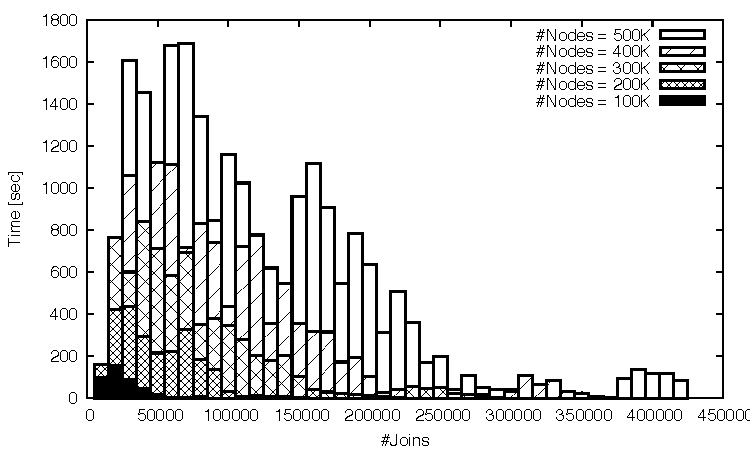
\includegraphics [width=0.80\linewidth]{fig2-cnm-joins-time-series.pdf}}
  \caption {ネットワークの解析に要した時間の時系列遷移}
  \label {fig: newman time diff}
\end{figure}

計算コストのボトルネックを調べるために、mixiネットワークの様々な部分集
合に対して解析を試みた。mixiはそれぞれのユーザーに対して、登録した順番
にIDナンバーを1から順番に与える。
$U= \{1,2,\ldots\}$
はユーザーIDの集合。
$F \subset U\times U$
は友人関係の集合とすると、mixiネットワークは、
$G_{\text {mixi}} = (U, F)$
のようなグラフで表せる。このグラフの部分集合を以下のように定義する。
%
\begin {align*}
  G_{\text {mixi}}^n = (U(n), F \cap (U(n) \times U(n))) \\
  \text {ただし } U(n) = \{ u \in U | u \le n \}
\end {align*}

図\ref {fig: newman time diff} はmixiネットワーク
の様々な部分集合$G_{\text {mixi}}^N (N = \text {100K}, \text {200K},
\text {300K}, \text {400K}, \text {500K})$に対
する、クラスタ抽出が完了するまでの解析に要した時間の時系列遷移である。
横軸は累積の合併の回数、縦軸は10,000回の合併に要する時間を秒で表してい
る。それぞれのデータセットでは、解析の前半で合併に要する時間がかかり、
後半で劇的に減少していることが分かる。

\cite{Clauset04}はCNM法の計算量が$O(md\text{log}n)$と述べている。
ここで$n$はノード数、$m$は全エッジ数、$d$はデンドログラムの高さである。
また、疎な社会ネットワークにおいて、$m$を$n$、$d$をlog$n$と近似でき、
計算量は$O(n\text{log}^2 n)$となると予想している。
一方、われわれの実験した実行時間の結果である図\ref{fig: newman time diff}のデータに対して
$f(x) = ax^b$を最小二乗近似した結果、$a = 1.51\cdot10^{-8} \pm2.06\cdot10^{-8}$,
$b = 2.13\pm0.104$と2次のオーダーで上昇することがわかった。これより$d\approx$log$n$の性質が少なくともmixiネットワークでは
現れないことがわかった。

われわれはデンドログラムがどのように成長するかを調べるため、合併履歴を
観察したところ、少数の巨大クラスタが、多数の小さなクラスタと合併するこ
とにより急速に成長していることが観測でき、この現象のために不均衡なデン
ドログラムが作られていることが分かった。

図\ref {fig: clauset ratio}は$G_{\text {mixi}}^{\text {500K}}$の解析プ
ロセスにおける各合併ごとの\emph {合併比率}を、片対数グラフにプロットし
た結果である。合併比率の定義を以下に示す。
\[\text{ratio}(c_{\text{i}},c_{\text{j}}) = \text{min}(|c_i|/|c_j|,|c_i|,|c_j|)\]%textは複数(乗算にしない)

\begin {figure}[htbp]
  \centerline {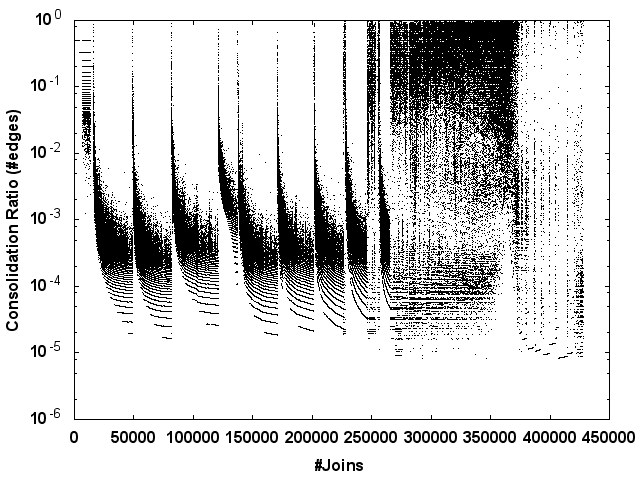
\includegraphics [width=0.80\linewidth]{fig3-cnm-ratio-join.png}}
  \caption {CNM法におけるクラスターの合併比率の推移(片対数)}
  \label {fig: clauset ratio}
\end{figure}

%\begin {空欄ブロック}{図3はn回目の合併を}
修正箇所:この個所を適切に書き換えなさい。
%\end {空欄ブロック}

不均衡な合併はデンドログラムの高さを成長させ、
\空欄 {修正箇所:この個所を適切に書き換えなさい}
ではなく、
\空欄 {修正箇所:この個所を適切に書き換えなさい}
となり
\空欄 {修正箇所:この個所を適切に書き換えなさい}
となる。


\section {提案手法}
\label {sect: algorithm}

前節ではCNM法の問題点を指摘した。本節ではCNM法の問
題点を改善し、速度を劇的に向上させる3つのヒューリスティックを提案する。

\begin {figure}
\begin {tabbing}
\hspace{.3\linewidth}\=$\mathrm {ratio}(c_i,c_j) \equiv \min(s(c_i)/s(c_j), s(c_j)/s(c_i))$; \\
\>\textbf {while} (\textbf {true}) \{\\
\>\quad\= updateDeltaQ(); \\
\>\>$\DQ \clustering {c_i} {c_j}\mathrm {ratio}(c_i,c_j)$が最大となる\\
\>\>\quad $(c_i, c_j) \in \clustering^2$を選択;\\
\>\>\textbf {if} ($\max(\DQ \clustering {c_i} {c_j} < 0$) \textbf {break};\\
\>\>\clustering\ := $\mathit {Join}(c_i, c_j)$;\\
\>\}
\end {tabbing}
  \caption {提案手法の概a略}
  \label {fig: tw algorithm}
\end {figure}

提案する手法を図\ref {fig: tw algorithm}に掲げる。全
体の構造はCNM法とほぼ同じである。異なるのは合併するクラスタの
対を決める戦略である。CNM法では$\DQ \clustering {c_i}
{c_j}$を用いていた。本手法ではそれに加えて合併比率($\mathrm
{ratio}(c_i, c_j)$)を用いる。このヒューリスティックは、合併の均衡を保ち、
平均したクラスタの成長を促すことにより、合併の不均衡による手法
の性能の劣化を抑えるように設計した。

さて、本稿ではここまでクラスタサイズ($|c_i|$)を定義してこなかった。ここ
で、3種類のクラスタサイズの定義を行うことにより、3種類のヒューリスティッ
クHE,HN,HE'を定義する。以下にそれぞれのヒューリスティックのクラスタサ
イズ$|c_i|$の定義を示す。

\begin{description}
	\item[HE]  $c_i$の隣接クラスタ数
	\item[HN]  $c_i$内のノード数
	\item[HE']  HEとCNM法を混同させた定義\footnote{詳細は \cite{Wakita07}をご覧ください。}
\end{description}


\section {評価}
\label {sect: evaluation}

\begin {空欄ブロック}{本節では、CNM法と前節で紹介した3種類の}
修正箇所:この個所を適切に書き換えなさい。
\end {空欄ブロック}

\begin {空欄ブロック}{4種類の手法を用い}
修正箇所:この個所を適切に書き換えなさい。
\end {空欄ブロック}

\begin{figure}[htbp]
\begin {空欄ブロック}{図5 実行時間比較}
修正箇所:この個所を適切に書き換えなさい。
\end {空欄ブロック}
\end{figure}

\begin {table}
  \caption {実行時間(秒)}
  \label {tbl: elapsed time}
  \begin {center}
    \begin {tabular}{lrrrrr} \\ \hline
          & 200K & 400K & 600K & 800K & 1M \\ \hline
      \textbf {CNM}& 2,530 & 11,800 & NA & NA & NA \\
      \textbf {HE}  & 129  & 408  & 814  & 1470 & 2170 \\
      \textbf {HE'} & 511  & 2,130 & 4,090 & 7,410 & 10,400 \\
      \textbf {HN}  & 25.7 & 70.0 & 123  & 190  & 268 \\
      \hline
    \end {tabular}
  \end {center}
\end {table}

\begin{figure}[htbp]
\begin {空欄ブロック}{図6 スケーラビリティ}
修正箇所:この個所を適切に書き換えなさい。
\end {空欄ブロック}
\end{figure}

\begin{figure}[htbp]
\begin {空欄ブロック}{図7 HNにおけるクラスターの}
修正箇所:この個所を適切に書き換えなさい。
\end {空欄ブロック}
\end{figure}

\begin {table}
\begin {空欄ブロック}{表2 モジュール性の比較}
修正箇所:この個所を適切に書き換えなさい。
\end {空欄ブロック}
\end {table}

\begin {空欄ブロック}{次にモジュール性の評価だが}
修正箇所:この個所を適切に書き換えなさい。
\end {空欄ブロック}

\begin {空欄ブロック}{HN法は、速度面において}
修正箇所:この個所を適切に書き換えなさい。
\end {空欄ブロック}

\begin {空欄ブロック}{図7にHNの}
修正箇所:この個所を適切に書き換えなさい。
\end {空欄ブロック}

\begin {空欄ブロック}{われわれはさらに}
修正箇所:この個所を適切に書き換えなさい。
\end {空欄ブロック}


\section {まとめ}
\label {sect: summary}

本研究では従来のClauset, Newman, Mooreが提案した手法のボトルネッ
クが合併の不均衡にあることを明らかにした。そして、3種類のヒューリスティッ
クを提案し、ボトルネックを取り除くことによって500万ノード以上のネットワー
クの解析も可能にした。

今後の課題としては、データ構造の改善によりより大規模なネットワークに対
する解析が可能になると考える。また、並列化を施すことにより、数億ノード
規模のネットワークに対する解析にも対応できると考えられる。

\subsection*{謝辞}

本研究の一部は文部科学省科学研究費助成金(18300041号)の援助を受けてい
ます。本稿の草稿について貴重なコメントをいただいた越田港さんに感謝しま
す。


\bibliographystyle {jplain} % 文献リストの書式の設定。jplainは最も標準的な書式です。
% pbibtex コマンドを用いて文献リストを作成するために、\bibliography コマンドで文献データベースを指定します。ここでは、references.bib という文献データベースを用いてリストを作成することを指示しています。

\begin{thebibliography}{10}

\bibitem{Cai04}
Deng~Cai, Xiaofei~He, Ji-Rong~Wen, and Wei-Ying Ma.
\newblock Block-level link analysis.
\newblock in {\em Proceedings of the 27th Annual International ACM SIGER Conference on Research and Development in Infornation Retrieval,}
\newblock SIGER '04, pp. 440-447, New York, NY, USA, 2004. ACM.

\bibitem{Clauset04}
A.~Clauset, M.~E.~J. Newman, and C.~Moore.
\newblock Finding community structure in very large networks.
\newblock {\em Physical Review E, Statistical, Nonlinear, and Soft Matter Physics}, Vol.~70, p. 066111, 2004.

\bibitem{Dean99}
Jeffery~Dean and Monika~R. Henzinger.
\newblock Finding related pages in the world wide web.
\newblock In {\em Computer Networks},Vol.~31, No.~11-16, pp. 1467--1479, 1999.

\bibitem{Gibson98}
David~Gibson, Jon~Kleinberg, and Prabhakar~Raghavan.
\newblock Inferring Web communities from link topology.
\newblock In {\em Proceedings of the Ninth ACM Conference on Hypertext and Hypermedia : Links, Objects, Time and Space — structure in Hypermedia Systems: Links, Objects, Time and Space—structure in Hypermedia Systems},
\newblock HYPERTEXT '98, pp.~225-234, New~York, NY, USA, 1998, ACM.

\bibitem{Kleinberg99}
Jon~M.~Kleinberg.
\newblock Authoritative sources in a hyperlinked environment.
\newblock {\em J.~ACM}, Vol.~46, No.~5, pp.~604-632, September 1999.

\bibitem{Kumar99}
Ravi~Kumar, Prabhakar~Raghavan, Sridhar~Rajagopalan, and Andrew~Tomkins.
\newblock Trawling the Web for emerging cyber-communities.
\newblock {\em Computer networks}, Vol.~31, No.~11, pp.~1481-1493, May 1999.

\bibitem{Miller01}
Joel~C.~Miller, Gregory~Rae, Fred~Schaefer, Lesley~A.~Ward, Thomas~LoFaro, and Ayman~Farahat.
\newblock Modifications of Kleinberg's HITS algorithm using matrix exponentiation and web log records.
\newblock In {\em Proceedings of the 24th Annual International ACM SIGER Conference on Research and Development in Information Retrieval},
\newblock SIGER '01, pp.~444-445, New~York, NY, USA, 2001, ACM.

\bibitem{Newman04}
M.~E.~J.~Newman and M.~Girvan.
\newblock Finding and evaluating community structure in net-works.
\newblock {\em Physical Review. E, Statistical, Nonlinear, and Soft Matter Physics}, Vol.~69, p.~026113 (16 pages), 2004

\bibitem{Onsjo06}
Mikael~Onsj\"o and Osamu~Watanabe.
\newblock A simple message passing algorithm for graph partitioning problems.
\newblock In Tetsuo~Asano, editor, {\em in Proceedings of 17th International symposium, ISAAC 2006}, Vol.~4288 of LNCS, pp.~507-516, Kolkata, India, December 2006, Springer.

\bibitem{Page99}
Lawrence~Page, Sergey~Brin, Rajev~Motwani, and Terry~Winograd.
\newblock The PageRank citation ranking: Bringing order to the Web.
\newblock Technical Report 1999-66, Stanford InfoLab, November 1999.

\bibitem{Toyoda01}
Masashi~Toyoda and Masaru~Kitsuregawa.
\newblock Creating a Web Community chart for navigating related communities.
\newblock In {\em Proceedings of the 12th ACM Conference on Hypertext and hypermedia}, HIPERTEXT '01, pp.~103-112. New~York, NY, USA, 2001, ACM.

\bibitem{Wakita07}
Ken~Wakita and Toshiyuki~Tsurumi.
\newblock Finding community structure in mega-scale social networks:[extended abstract].
\newblock In {\em Proceedings of the 16th international conference on World Wide Web}, pp.~1275-1276. ACM, 2007.

\bibitem{Wu04}
Fang~Wu and Bernardo~A~Huberman.
\newblock Finding communities in linear time: a physics approach.
\newblock {\em The European Physical Journal B-Condensed Matter and Complex Systems}, Vol.~38, No.~2, pp.~331-338, 2004.

\end {thebibliography}


\bibliography {references}

\end {document}
